\documentclass[
  doc,
  floatsintext,
  longtable,
  a4paper,
  nolmodern,
  notxfonts,
  notimes,
  colorlinks=true,linkcolor=blue,citecolor=blue,urlcolor=blue]{apa7}

\usepackage{amsmath}
\usepackage{amssymb}

\geometry{inner=1in, outer=1in}
\fancyhfoffset[LE,RO]{0cm}


\usepackage[bidi=default]{babel}
\babelprovide[main,import]{spanish}
\StartBabelCommands{spanish}{captions} [unicode, fontenc=TU EU1 EU2, charset=utf8] \SetString{\keywordname}{Palabras
Claves}
\EndBabelCommands


% get rid of language-specific shorthands (see #6817):
\let\LanguageShortHands\languageshorthands
\def\languageshorthands#1{}

\RequirePackage{longtable}
\RequirePackage{threeparttablex}

\makeatletter
\renewcommand{\paragraph}{\@startsection{paragraph}{4}{\parindent}%
	{0\baselineskip \@plus 0.2ex \@minus 0.2ex}%
	{-.5em}%
	{\normalfont\normalsize\bfseries\typesectitle}}

\renewcommand{\subparagraph}[1]{\@startsection{subparagraph}{5}{0.5em}%
	{0\baselineskip \@plus 0.2ex \@minus 0.2ex}%
	{-\z@\relax}%
	{\normalfont\normalsize\bfseries\itshape\hspace{\parindent}{#1}\textit{\addperi}}{\relax}}
\makeatother




\usepackage{longtable, booktabs, multirow, multicol, colortbl, hhline, caption, array, float, xpatch}
\usepackage{subcaption}


\renewcommand\thesubfigure{\Alph{subfigure}}
\setcounter{topnumber}{2}
\setcounter{bottomnumber}{2}
\setcounter{totalnumber}{4}
\renewcommand{\topfraction}{0.85}
\renewcommand{\bottomfraction}{0.85}
\renewcommand{\textfraction}{0.15}
\renewcommand{\floatpagefraction}{0.7}

\usepackage{tcolorbox}
\tcbuselibrary{listings,theorems, breakable, skins}
\usepackage{fontawesome5}

\definecolor{quarto-callout-color}{HTML}{909090}
\definecolor{quarto-callout-note-color}{HTML}{0758E5}
\definecolor{quarto-callout-important-color}{HTML}{CC1914}
\definecolor{quarto-callout-warning-color}{HTML}{EB9113}
\definecolor{quarto-callout-tip-color}{HTML}{00A047}
\definecolor{quarto-callout-caution-color}{HTML}{FC5300}
\definecolor{quarto-callout-color-frame}{HTML}{ACACAC}
\definecolor{quarto-callout-note-color-frame}{HTML}{4582EC}
\definecolor{quarto-callout-important-color-frame}{HTML}{D9534F}
\definecolor{quarto-callout-warning-color-frame}{HTML}{F0AD4E}
\definecolor{quarto-callout-tip-color-frame}{HTML}{02B875}
\definecolor{quarto-callout-caution-color-frame}{HTML}{FD7E14}

%\newlength\Oldarrayrulewidth
%\newlength\Oldtabcolsep


\usepackage{hyperref}




\providecommand{\tightlist}{%
  \setlength{\itemsep}{0pt}\setlength{\parskip}{0pt}}
\usepackage{longtable,booktabs,array}
\usepackage{calc} % for calculating minipage widths
% Correct order of tables after \paragraph or \subparagraph
\usepackage{etoolbox}
\makeatletter
\patchcmd\longtable{\par}{\if@noskipsec\mbox{}\fi\par}{}{}
\makeatother
% Allow footnotes in longtable head/foot
\IfFileExists{footnotehyper.sty}{\usepackage{footnotehyper}}{\usepackage{footnote}}
\makesavenoteenv{longtable}

\usepackage{graphicx}
\makeatletter
\newsavebox\pandoc@box
\newcommand*\pandocbounded[1]{% scales image to fit in text height/width
  \sbox\pandoc@box{#1}%
  \Gscale@div\@tempa{\textheight}{\dimexpr\ht\pandoc@box+\dp\pandoc@box\relax}%
  \Gscale@div\@tempb{\linewidth}{\wd\pandoc@box}%
  \ifdim\@tempb\p@<\@tempa\p@\let\@tempa\@tempb\fi% select the smaller of both
  \ifdim\@tempa\p@<\p@\scalebox{\@tempa}{\usebox\pandoc@box}%
  \else\usebox{\pandoc@box}%
  \fi%
}
% Set default figure placement to htbp
\def\fps@figure{htbp}
\makeatother







\usepackage{newtx}

\defaultfontfeatures{Scale=MatchLowercase}
\defaultfontfeatures[\rmfamily]{Ligatures=TeX,Scale=1}





\title{Modelos Económicos: Clásico y Keynesiano}


\shorttitle{Modelos Económicos}


\usepackage{etoolbox}


\course{Economía Matemática I}
\professor{Econ. Yupanqui Pillhuaman, William}
\duedate{14/04/2025}

\ccoppy{\textcopyright~2025}



\author{Edison Achalma}



\affiliation{
{Escuela Profesional de Economía, Universidad Nacional de San Cristóbal
de Huamanga}}




\leftheader{Achalma}

\date{2025-04-14}


\abstract{This article examines the Walrasian equilibrium within
classical and Keynesian economic models, focusing on the effects of
nominal and real rigidities. It presents the assumptions, equations, and
policy analyses for the classical model with flexible prices and wages,
the Keynesian model with nominal wage rigidity, and models incorporating
real and nominal rigidities. Using differential calculus and matrix
representations, the study analyzes the impact of fiscal and monetary
policies on real and nominal variables, such as output, employment,
interest rates, and prices. The classical model demonstrates money
neutrality and ineffective fiscal policies due to price flexibility,
while the Keynesian model highlights unemployment and effective policy
interventions under rigidities. The analysis provides a comprehensive
understanding of economic equilibrium dynamics for students and
researchers in mathematical economics. }

\keywords{keyword1, keyword2}

\authornote{\par{\addORCIDlink{Edison Achalma}{0000-0001-6996-3364}} 
\par{ }
\par{   El autor no tiene conflictos de interés que revelar.    Los
roles de autor se clasificaron utilizando la taxonomía de roles de
colaborador (CRediT; https://credit.niso.org/) de la siguiente
manera:  Edison Achalma:   conceptualización, redacción}
\par{La correspondencia relativa a este artículo debe dirigirse a Edison
Achalma, Email: \href{mailto:elmer.achalma.09@unsch.edu.pe}{elmer.achalma.09@unsch.edu.pe}}
}

\makeatletter
\let\endoldlt\endlongtable
\def\endlongtable{
\hline
\endoldlt
}
\makeatother

\urlstyle{same}



\makeatletter
\@ifpackageloaded{caption}{}{\usepackage{caption}}
\AtBeginDocument{%
\ifdefined\contentsname
  \renewcommand*\contentsname{Tabla de contenidos}
\else
  \newcommand\contentsname{Tabla de contenidos}
\fi
\ifdefined\listfigurename
  \renewcommand*\listfigurename{List of Figures}
\else
  \newcommand\listfigurename{List of Figures}
\fi
\ifdefined\listtablename
  \renewcommand*\listtablename{List of Tables}
\else
  \newcommand\listtablename{List of Tables}
\fi
\ifdefined\figurename
  \renewcommand*\figurename{Figura}
\else
  \newcommand\figurename{Figura}
\fi
\ifdefined\tablename
  \renewcommand*\tablename{Tabla}
\else
  \newcommand\tablename{Tabla}
\fi
}
\@ifpackageloaded{float}{}{\usepackage{float}}
\floatstyle{ruled}
\@ifundefined{c@chapter}{\newfloat{codelisting}{h}{lop}}{\newfloat{codelisting}{h}{lop}[chapter]}
\floatname{codelisting}{Listing}
\newcommand*\listoflistings{\listof{codelisting}{List of Listings}}
\makeatother
\makeatletter
\@ifpackageloaded{tikz}{}{\usepackage{tikz}}
\makeatother
\makeatletter
\@ifpackageloaded{caption}{}{\usepackage{caption}}
\@ifpackageloaded{subcaption}{}{\usepackage{subcaption}}
\makeatother
\makeatletter
\@ifpackageloaded{fontawesome5}{}{\usepackage{fontawesome5}}
\makeatother

% From https://tex.stackexchange.com/a/645996/211326
%%% apa7 doesn't want to add appendix section titles in the toc
%%% let's make it do it
\makeatletter
\xpatchcmd{\appendix}
  {\par}
  {\addcontentsline{toc}{section}{\@currentlabelname}\par}
  {}{}
\makeatother

%% Disable longtable counter
%% https://tex.stackexchange.com/a/248395/211326

\usepackage{etoolbox}

\makeatletter
\patchcmd{\LT@caption}
  {\bgroup}
  {\bgroup\global\LTpatch@captiontrue}
  {}{}
\patchcmd{\longtable}
  {\par}
  {\par\global\LTpatch@captionfalse}
  {}{}
\apptocmd{\endlongtable}
  {\ifLTpatch@caption\else\addtocounter{table}{-1}\fi}
  {}{}
\newif\ifLTpatch@caption
\makeatother

\begin{document}

\maketitle

\hypertarget{toc}{}
\tableofcontents
\newpage
\section[Introduction]{Modelos Económicos}

\setcounter{secnumdepth}{5}

\setlength\LTleft{0pt}


\section{Modelo Clásico: Equilibrio de
Walras}\label{modelo-cluxe1sico-equilibrio-de-walras}

\subsection{Supuestos}\label{supuestos}

\begin{itemize}
\tightlist
\item
  \textbf{Precios y salarios flexibles:} \(W\) y \(P\), \(W/P\) salario
  real.
\item
  \textbf{Todos los mercados en equilibrio:}

  \begin{itemize}
  \tightlist
  \item
    \(Y^t = Y^d = Y^s\): Equilibrio en el mercado de bienes.
  \item
    \(M^d = M^s\): Equilibrio en el mercado monetario.
  \item
    \(N^t = N^d = N^s\): Equilibrio en el mercado de trabajo.
  \end{itemize}
\item
  \textbf{Pleno empleo.}
\item
  \textbf{Desempleo voluntario.}
\item
  \textbf{Demanda agregada:} Deducida de la teoría cuantitativa del
  dinero.
\item
  \textbf{Oferta agregada:} Deducida del mercado de trabajo por los
  salarios reales y nivel de precios, tiene forma perfectamente
  inelástica.
\end{itemize}

\subsection{Observaciones}\label{observaciones}

\begin{itemize}
\tightlist
\item
  \textbf{Variables reales:} Producción (\(Y^t\)) y nivel de empleo
  (\(N^t\)).
\item
  \textbf{Variables nominales:} Tasa de interés (\(r\)) y precios
  (\(P\)).
\item
  \textbf{Neutralidad del dinero:} Un aumento en la oferta monetaria
  (\(\uparrow M\)) implica un aumento proporcional en los precios
  (\(\uparrow P\)), sin afectar las variables reales (\(Y^t, N^t\)).
\item
  \textbf{Políticas fiscales y de renta:} Ineficientes debido al ajuste
  automático de precios y salarios.
\end{itemize}

\subsection{Planteamiento}\label{planteamiento}

\begin{enumerate}
\def\labelenumi{\arabic{enumi}.}
\item
  \textbf{Planteamiento del modelo:}

  \[
  \begin{aligned}
  Y^t &= C(Y^t) + I(r - \bar{\pi}) + \bar{\mathrm{SD}}, & \bar{\mathrm{SD}} &= \bar{C} + \bar{G} + \bar{I}, \\
  \frac{\bar{M}}{P} &= L(Y^t, r), \\
  N^t &= N^d \left( \frac{W}{P} \right), \\
  N^t &= N^s \left( \frac{W}{P} \right), \\
  Y^t &= f(N^t),
  \end{aligned}
  \]

  donde:

  \begin{itemize}
  \tightlist
  \item
    \textbf{Variables endógenas:} \(Y^t\), \(r\), \(N^t\),
    \(\frac{W}{P}\), \(P\).
  \item
    \textbf{Variables exógenas:} \(\bar{\mathrm{SD}}\), \(\bar{M}\),
    \(\bar{\pi}\).
  \end{itemize}
\item
  \textbf{Forma de identidad:}

  \[
  \begin{aligned}
  Y^t - C(Y^t) - I(r - \bar{\pi}) - \bar{\mathrm{SD}} &= 0 & &\leftrightarrow \bar{Y}^t = Y^t(\bar{\mathrm{SD}}, \bar{M}, \bar{\pi}), \\
  \frac{\bar{M}}{P} - L(Y^t, r) &= 0 & &\leftrightarrow \bar{r} = r(\bar{\mathrm{SD}}, \bar{M}, \bar{\pi}), \\
  N^t - N^d \left( \frac{W}{P} \right) &= 0 & &\leftrightarrow \bar{N}^t = N^t(\bar{\mathrm{SD}}, \bar{M}, \bar{\pi}), \\
  N^t - N^s \left( \frac{W}{P} \right) &= 0 & &\leftrightarrow \bar{\frac{W}{P}} = \frac{W}{P}(\bar{\mathrm{SD}}, \bar{M}, \bar{\pi}), \\
  Y^t - f(N^t) &= 0 & &\leftrightarrow \bar{P} = P(\bar{\mathrm{SD}}, \bar{M}, \bar{\pi}),
  \end{aligned}
  \]
\item
  \textbf{Aplicación de diferencial total:}

  \[
  \begin{aligned}
  (1 - C_{Y^t}) dY^t - I_r dr &= -I_r d\bar{\pi} + d\bar{\mathrm{SD}}, \\
  -L_{Y^t} dY^t + L_r dr + \frac{\bar{M}}{P^2} dP &= \frac{d\bar{M}}{P}, \\
  dN^t &= N^d_{\frac{W}{P}} d \left( \frac{W}{P} \right), \\
  dN^t &= N^s_{\frac{W}{P}} d \left( \frac{W}{P} \right), \\
  dY^t &= f'(N^t) dN^t.
  \end{aligned}
  \]
\item
  \textbf{Despejando exógenas:}

  \[
  \begin{aligned}
  (1 - C_{Y^t}) dY^t - I_r dr &= -I_r d\bar{\pi} + d\bar{\mathrm{SD}}, \\
  -L_{Y^t} dY^t + L_r dr - \frac{\bar{M}}{P^2} dP &= -\frac{d\bar{M}}{P}, \\
  dN^t - N^d_{\frac{W}{P}} d \left( \frac{W}{P} \right) &= 0, \\
  dN^t - N^s_{\frac{W}{P}} d \left( \frac{W}{P} \right) &= 0, \\
  dY^t - f'(N^t) dN^t &= 0.
  \end{aligned}
  \]
\item
  \textbf{Matrices:}

  \[
  \begin{bmatrix}
  1 - C_{Y^t} & -I_r & 0 & 0 & 0 \\
  -L_{Y^t} & L_r & -\frac{\bar{M}}{P^2} & 0 & 0 \\
  0 & 0 & 0 & 1 & -N^d_{\frac{W}{P}} \\
  0 & 0 & 0 & 1 & -N^s_{\frac{W}{P}} \\
  1 & 0 & 0 & -f'(N^t) & 0
  \end{bmatrix}
  \begin{bmatrix}
  dY^t \\
  dr \\
  dP \\
  dN^t \\
  d \left( \frac{W}{P} \right)
  \end{bmatrix}
  =
  \begin{bmatrix}
  1 & 0 & -I_r \\
  0 & -\frac{1}{P} & 0 \\
  0 & 0 & 0 \\
  0 & 0 &-I_r \\
  0 & 0 & 0
  \end{bmatrix}
  \begin{bmatrix}
  d\bar{\mathrm{SD}} \\
  d\bar{M} \\
  d\bar{\pi}
  \end{bmatrix}.
  \]
\item
  \textbf{Determinante:}

  Calculamos el determinante de la matriz para evaluar la estabilidad
  del sistema:

  \[
  \det \begin{bmatrix}
  1 - C_{Y^t} & -I_r & 0 & 0 & 0 \\
  -L_{Y^t} & L_r & -\frac{\bar{M}}{P^2} & 0 & 0 \\
  0 & 0 & 0 & 1 & -N^d_{\frac{W}{P}} \\
  0 & 0 & 0 & 1 & -N^s_{\frac{W}{P}} \\
  1 & 0 & 0 & -f'(N^t) & 0
  \end{bmatrix} = \frac{\bar{M} I_r}{P^2} \left( N^d_{\frac{W}{P}} - N^s_{\frac{W}{P}} \right).
  \]

  El determinante no es cero, lo que indica que el sistema es invertible
  y tiene solución única bajo las condiciones del modelo.
\item
  \textbf{Análisis de política fiscal:}

  Consideramos el efecto de \(d\bar{\mathrm{SD}} > 0\), con
  \(d\bar{M} = 0\), \(d\bar{\pi} = 0\):

  \[
  \begin{bmatrix}
  1 - C_{Y^t} & -I_r & 0 & 0 & 0 \\
  -L_{Y^t} & L_r & -\frac{\bar{M}}{P^2} & 0 & 0 \\
  0 & 0 & 0 & 1 & -N^d_{\frac{W}{P}} \\
  0 & 0 & 0 & 1 & -N^s_{\frac{W}{P}} \\
  1 & 0 & 0 & -f'(N^t) & 0
  \end{bmatrix}
  \begin{bmatrix}
  \frac{dY^t}{d\bar{\mathrm{SD}}} \\
  \frac{dr}{d\bar{\mathrm{SD}}} \\
  \frac{dP}{d\bar{\mathrm{SD}}} \\
  \frac{dN^t}{d\bar{\mathrm{SD}}} \\
  \frac{d \left( \frac{W}{P} \right)}{d\bar{\mathrm{SD}}}
  \end{bmatrix}
  = \begin{bmatrix}
  1 \\
  0 \\
  0 \\
  0 \\
  0
  \end{bmatrix}.
  \]

  Calculamos:

  \[
  \frac{dY^t}{d\bar{\mathrm{SD}}} = \frac{\det \begin{bmatrix}
  1 & -I_r & 0 & 0 & 0 \\
  0 & L_r & -\frac{\bar{M}}{P^2} & 0 & 0 \\
  0 & 0 & 0 & 1 & -N^d_{\frac{W}{P}} \\
  0 & 0 & 0 & 1 & -N^s_{\frac{W}{P}} \\
  0 & 0 & 0 & -f'(N^t) & 0
  \end{bmatrix}}{\det \begin{bmatrix}
  1 - C_{Y^t} & -I_r & 0 & 0 & 0 \\
  -L_{Y^t} & L_r & -\frac{\bar{M}}{P^2} & 0 & 0 \\
  0 & 0 & 0 & 1 & -N^d_{\frac{W}{P}} \\
  0 & 0 & 0 & 1 & -N^s_{\frac{W}{P}} \\
  1 & 0 & 0 & -f'(N^t) & 0
  \end{bmatrix}}.
  \]

  Numerador:

  \[
  \det \begin{bmatrix}
  1 & -I_r & 0 & 0 & 0 \\
  0 & L_r & -\frac{\bar{M}}{P^2} & 0 & 0 \\
  0 & 0 & 0 & 1 & -N^d_{\frac{W}{P}} \\
  0 & 0 & 0 & 1 & -N^s_{\frac{W}{P}} \\
  0 & 0 & 0 & -f'(N^t) & 0
  \end{bmatrix} = 0 \quad (\text{primera columna tiene ceros en filas 2--5, y el bloque } 3 \times 3 \text{ da } 0).
  \]

  Denominador:

  \[
  \det \begin{bmatrix}
  1 - C_{Y^t} & -I_r & 0 & 0 & 0 \\
  -L_{Y^t} & L_r & -\frac{\bar{M}}{P^2} & 0 & 0 \\
  0 & 0 & 0 & 1 & -N^d_{\frac{W}{P}} \\
  0 & 0 & 0 & 1 & -N^s_{\frac{W}{P}} \\
  1 & 0 & 0 & -f'(N^t) & 0
  \end{bmatrix} = \frac{\bar{M} I_r}{P^2} \left( N^d_{\frac{W}{P}} - N^s_{\frac{W}{P}} \right) \neq 0.
  \]

  Resultado:

  \[
  \frac{dY^t}{d\bar{\mathrm{SD}}} = \frac{0}{\frac{\bar{M} I_r}{P^2} \left( N^d_{\frac{W}{P}} - N^s_{\frac{W}{P}} \right)} = 0.
  \]

  Esto indica que un aumento en \(d\bar{\mathrm{SD}}\) no afecta
  \(Y^t\), consistente con el modelo clásico, donde el pleno empleo y la
  flexibilidad de precios neutralizan la política fiscal, afectando solo
  variables nominales.
\end{enumerate}

\subsection{Efecto crowding out}\label{efecto-crowding-out}

Un aumento en el gasto público (\(G\)) incrementa \(Y^d\), lo que
inicialmente eleva \(Y^t\). Esto aumenta la demanda de dinero
(\(M^d > M^s\)), elevando la tasa de interés (\(r\)) y reduciendo la
inversión (\(I\)). En el modelo clásico, \(Y^t\) regresa a un nivel
menor por el ajuste de precios, pero con una tasa de interés más alta:

\[
G \uparrow \rightarrow Y^d \uparrow \rightarrow Y^t \uparrow \rightarrow M^d > M^s \rightarrow r \uparrow \rightarrow I \downarrow.
\]

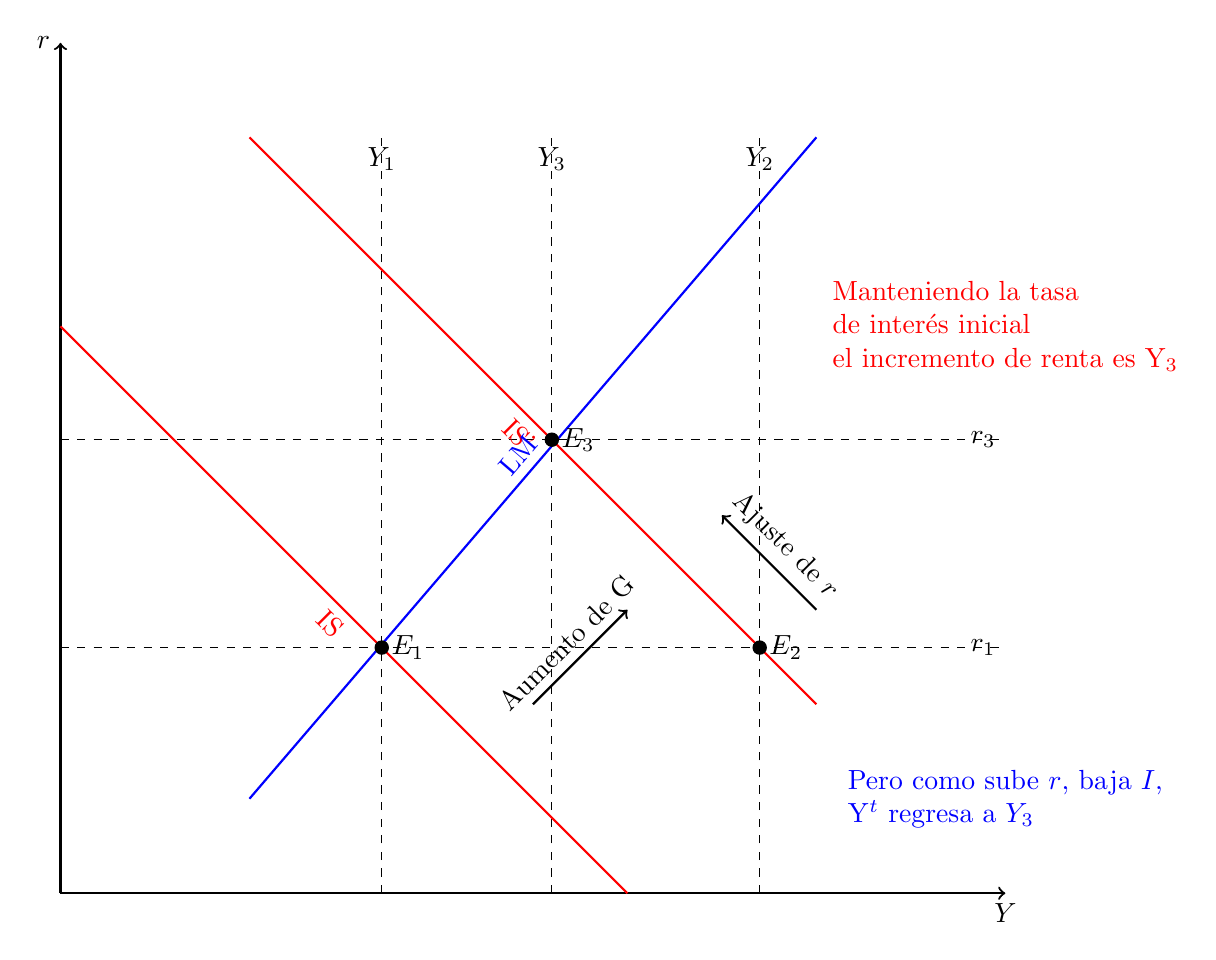
\begin{tikzpicture}[scale=1.2]
% Ejes
\draw[->, thick] (0,0) -- (10,0) node[below] {$Y$}; % Eje Y
\draw[->, thick] (0,0) -- (0,9) node[left] {$r$}; % Eje r
% Líneas de cuadrícula (punteadas)
\draw[dashed] (0,2.6) -- (10,2.6) node[left] {$r_1$};
\draw[dashed] (0,4.8) -- (10,4.8) node[left] {$r_3$};
\draw[dashed] (3.4,0) -- (3.4,8) node[below] {$Y_1$};
\draw[dashed] (5.2,0) -- (5.2,8) node[below] {$Y_3$};
\draw[dashed] (7.4,0) -- (7.4,8) node[below] {$Y_2$};
% Curva IS inicial
\draw[red, thick] (0,6) -- (6,0) node[midway, below, sloped] {IS};
% Curva IS desplazada
\draw[red, thick] (2,8) -- (8,2) node[midway, below, sloped] {IS'};
% Curva LM (pendiente positiva)
\draw[blue, thick] (2,1) -- (8,8) node[midway, above, sloped] {LM};
% Puntos de equilibrio
\filldraw (3.4,2.6) circle (2pt) node[right] {$E_1$}; % (Y_0, r_0), intersección IS y LM
\filldraw (7.4,2.6) circle (2pt) node[right] {$E_2$}; % (Y_2, r_1), en IS' con r_1 = r_0
\filldraw (5.2,4.8) circle (2pt) node[right] {$E_3$}; % (Y_3, r_2), intersección IS' y LM
% Flechas de desplazamiento
% Paralela a LM (pendiente positiva) para el desplazamiento de IS
\draw[->, thick] (5,2) -- (6,3) node[midway, above, sloped] {Aumento de \(\mathrm{G}\)};
% Paralela a IS (pendiente negativa) para el ajuste de r
\draw[->, thick] (8,3) -- (7,4) node[midway, above, sloped] {Ajuste de \(r\)};
% Anotaciones
\node[align=left, red] at (10,6) {Manteniendo la tasa \\ de interés inicial \\ el incremento de renta es \(\mathrm{Y}_3\) };
\node[align=left, blue] at (10,1) {Pero como sube \(r\), baja \(I\), \\ \(\mathrm{Y}^t\) regresa a \(Y_3\)};
\end{tikzpicture}


Si no hay cambio en el tipo de interés, no hay efecto expansivo.

\section{Modelo 2: Salarios Nominales Rígidos
(Keynesiano)}\label{modelo-2-salarios-nominales-ruxedgidos-keynesiano}

\subsection{Supuestos}\label{supuestos-1}

\begin{itemize}
\tightlist
\item
  \textbf{Salario nominal rígido:} \(\bar{W}\) es exógeno.
\item
  \textbf{Equilibrio en el mercado de bienes.}
\item
  \textbf{Equilibrio en el mercado monetario.}
\item
  \textbf{Desequilibrio en el mercado de trabajo:} Oferta de trabajo
  (\(N^s\)) mayor a la demanda de trabajo (\(N^d\)).
\end{itemize}

\[
N^s > N^d \quad (\text{exceso de oferta de trabajo})
\]

\begin{itemize}
\tightlist
\item
  \textbf{Desempleo involuntario.}
\item
  \textbf{Oferta agregada:} Deducida de la curva de Phillips.
\item
  \textbf{Empleo efectivo:} Determinado por la demanda de trabajo,
  \(N^t = N^d\).
\item
  \textbf{Alto desempleo:} \(\frac{dN}{dW} < 0\).
\end{itemize}

\subsection{Planteamiento}\label{planteamiento-1}

\begin{enumerate}
\def\labelenumi{\arabic{enumi}.}
\item
  \textbf{Planteamiento del modelo:}

  \[
  \begin{aligned}
  Y^t &= C(Y^t) + I(r - \bar{\pi}) + \bar{\mathrm{SD}}, & \bar{\mathrm{SD}} &= \bar{C} + \bar{G} + \bar{I}, \\
  \frac{\bar{M}}{P} &= L(Y^t, r), \\
  N^t &= N^d \left( \frac{\bar{W}}{P} \right), \\
  Y^t &= f(N^t),
  \end{aligned}
  \]

  donde:

  \begin{itemize}
  \tightlist
  \item
    \textbf{Variables endógenas:} \(Y^t\), \(r\), \(N^t\), \(P\).
  \item
    \textbf{Variables exógenas:} \(\bar{\mathrm{SD}}\), \(\bar{M}\),
    \(\bar{\pi}\), \(\bar{W}\).
  \end{itemize}
\item
  \textbf{Forma de identidad:}

  \[
  \begin{aligned}
  Y^t - C(Y^t) - I(r - \bar{\pi}) - \bar{\mathrm{SD}} &= 0 & &\leftrightarrow Y^{t*} = Y^t(\bar{\mathrm{SD}}, \bar{M}, \bar{\pi}, \bar{W}), \\
  \frac{\bar{M}}{P} - L(Y^t, r) &= 0 & &\leftrightarrow r^* = r(\bar{\mathrm{SD}}, \bar{M}, \bar{\pi}, \bar{W}), \\
  N^t - N^d \left( \frac{\bar{W}}{P} \right) &= 0 & &\leftrightarrow N^{t*} = N^t(\bar{\mathrm{SD}}, \bar{M}, \bar{\pi}, \bar{W}), \\
  Y^t - f(N^t) &= 0 & &\leftrightarrow P^* = P(\bar{\mathrm{SD}}, \bar{M}, \bar{\pi}, \bar{W}),
  \end{aligned}
  \]
\item
  \textbf{Aplicando diferenciales:}

  \[
  \begin{aligned}
  (1 - C_{Y^t}) dY^t - I_r dr &= d\bar{\mathrm{SD}} + I_r d\bar{\pi}, \\
  -L_{Y^t} dY^t - L_r dr + \frac{\bar{M}}{P^2} dP &= \frac{d\bar{M}}{P}, \\
  dN^t - N^d_{\frac{\bar{W}}{P}} \left( \frac{d\bar{W}}{P} - \frac{\bar{W}}{P^2} dP \right) &= 0, \\
  dY^t - f'(N^t) dN^t &= 0.
  \end{aligned}
  \]
\item
  \textbf{Despejando exógenas:}

  \[
  \begin{aligned}
  (1 - C_{Y^t}) dY^t - I_r dr &= d\bar{\mathrm{SD}} + I_r d\bar{\pi}, \\
  -L_{Y^t} dY^t - L_r dr - \frac{\bar{M}}{P^2} dP &= -\frac{d\bar{M}}{P}, \\
  dN^t + N^d_{\frac{\bar{W}}{P}} \left( \frac{\bar{W}}{P^2} dP \right) &= N^d_{\frac{\bar{W}}{P}} \left( \frac{d\bar{W}}{P} \right), \\
  dY^t - f'(N^t) dN^t &= 0.
  \end{aligned}
  \]
\item
  \textbf{Matrices:}

  \[
  \begin{bmatrix}
  1 - C_{Y^t} & -I_r & 0 & 0 \\
  -L_{Y^t} & -L_r & -\frac{\bar{M}}{P^2} & 0 \\
  0 & 0 & N^d_{\frac{\bar{W}}{P}} \frac{\bar{W}}{P^2} & 1 \\
  1 & 0 & 0 & -f'(N^t)
  \end{bmatrix}
  \begin{bmatrix}
  dY^t \\
  dr \\
  dP \\
  dN^t
  \end{bmatrix}
  =
  \begin{bmatrix}
  1 & 0 & I_r & 0 \\
  0 & -\frac{1}{P} & 0 & 0 \\
  0 & 0 & 0 & N^d_{\frac{\bar{W}}{P}} \frac{1}{P} \\
  0 & 0 & 0 & 0
  \end{bmatrix}
  \begin{bmatrix}
  d\bar{\mathrm{SD}} \\
  d\bar{M} \\
  d\bar{\pi} \\
  d\bar{W}
  \end{bmatrix}.
  \]
\item
  \textbf{Cálculo del determinante:}

  \[
  \Delta = \begin{vmatrix}
  1 - C_{Y^t} & -I_r & 0 & 0 \\
  -L_{Y^t} & -L_r & -\frac{\bar{M}}{P^2} & 0 \\
  0 & 0 & N^d_{\frac{\bar{W}}{P}} \frac{\bar{W}}{P^2} & 1 \\
  1 & 0 & 0 & -f'(N^t)
  \end{vmatrix}.
  \]

  Expandiendo por la cuarta fila:

  \[
  \Delta = (-f'(N^t)) \cdot (-1)^{4+4} \det \begin{bmatrix}
  1 - C_{Y^t} & -I_r & 0 \\
  -L_{Y^t} & -L_r & -\frac{\bar{M}}{P^2} \\
  0 & 0 & N^d_{\frac{\bar{W}}{P}} \frac{\bar{W}}{P^2}
  \end{bmatrix}
  + 1 \cdot (-1)^{4+3} \det \begin{bmatrix}
  1 - C_{Y^t} & -I_r & 0 \\
  -L_{Y^t} & -L_r & -\frac{\bar{M}}{P^2} \\
  1 & 0 & 0
  \end{bmatrix}.
  \]

  El segundo determinante es:

  \[
  \det \begin{bmatrix}
  1 - C_{Y^t} & -I_r & 0 \\
  -L_{Y^t} & -L_r & -\frac{\bar{M}}{P^2} \\
  1 & 0 & 0
  \end{bmatrix} = -I_r \frac{\bar{M}}{P^2}.
  \]

  El primer determinante es:

  \[
  \det \begin{bmatrix}
  1 - C_{Y^t} & -I_r & 0 \\
  -L_{Y^t} & -L_r & -\frac{\bar{M}}{P^2} \\
  0 & 0 & N^d_{\frac{\bar{W}}{P}} \frac{\bar{W}}{P^2}
  \end{bmatrix} = N^d_{\frac{\bar{W}}{P}} \frac{\bar{W}}{P^2} \det \begin{bmatrix}
  1 - C_{Y^t} & -I_r \\
  -L_{Y^t} & -L_r
  \end{bmatrix}.
  \]

  Calculando:

  \[
  \det \begin{bmatrix}
  1 - C_{Y^t} & -I_r \\
  -L_{Y^t} & -L_r
  \end{bmatrix} = (1 - C_{Y^t})(-L_r) - (-I_r)(-L_{Y^t}) = -L_r (1 - C_{Y^t}) - I_r L_{Y^t}.
  \]

  Entonces:

  \[
  \Delta = -f'(N^t) \cdot N^d_{\frac{\bar{W}}{P}} \frac{\bar{W}}{P^2} \left[ -L_r (1 - C_{Y^t}) - I_r L_{Y^t} \right] - I_r \frac{\bar{M}}{P^2}.
  \]

  Factorizando:

  \[
  \Delta = \frac{\bar{M} I_r}{P^2} - f'(N^t) N^d_{\frac{\bar{W}}{P}} \frac{\bar{W}}{P^2} \left[ L_r (1 - C_{Y^t}) + I_r L_{Y^t} \right].
  \]

  Dado que \(L_r < 0\), \(I_r < 0\), \(1 - C_{Y^t} > 0\),
  \(L_{Y^t} > 0\), \(f'(N^t) > 0\), \(N^d_{\frac{\bar{W}}{P}} < 0\),
  \(\bar{M} > 0\), \(P > 0\), el signo de \(\Delta\) depende de los
  valores, pero típicamente \(\Delta < 0\).
\item
  \textbf{Análisis de política fiscal:}

  Consideramos \(\frac{dN^t}{d\bar{W}}\), con \(d\bar{W} \neq 0\),
  \(d\bar{\mathrm{SD}} = 0\), \(d\bar{\pi} = 0\), \(d\bar{M} = 0\):

  \[
  \begin{bmatrix}
  1 - C_{Y^t} & -I_r & 0 & 0 \\
  -L_{Y^t} & -L_r & -\frac{\bar{M}}{P^2} & 0 \\
  0 & 0 & N^d_{\frac{\bar{W}}{P}} \frac{\bar{W}}{P^2} & 1 \\
  1 & 0 & 0 & -f'(N^t)
  \end{bmatrix}
  \begin{bmatrix}
  \frac{dY^t}{d\bar{W}} \\
  \frac{dr}{d\bar{W}} \\
  \frac{dP}{d\bar{W}} \\
  \frac{dN^t}{d\bar{W}}
  \end{bmatrix}
  =
  \begin{bmatrix}
  0 \\
  0 \\
  N^d_{\frac{\bar{W}}{P}} \frac{1}{P} \\
  0
  \end{bmatrix}.
  \]

  Calculamos \(\frac{dN^t}{d\bar{W}}\) usando el método de Cramer:

  \[
  \frac{dN^t}{d\bar{W}} = \frac{\det \begin{bmatrix}
  1 - C_{Y^t} & -I_r & 0 & 0 \\
  -L_{Y^t} & -L_r & -\frac{\bar{M}}{P^2} & 0 \\
  0 & 0 & N^d_{\frac{\bar{W}}{P}} \frac{\bar{W}}{P^2} & N^d_{\frac{\bar{W}}{P}} \frac{1}{P} \\
  1 & 0 & 0 & 0
  \end{bmatrix}}{\Delta}.
  \]

  Numerador:

  \[
  \det \begin{bmatrix}
  1 - C_{Y^t} & -I_r & 0 & 0 \\
  -L_{Y^t} & -L_r & -\frac{\bar{M}}{P^2} & 0 \\
  0 & 0 & N^d_{\frac{\bar{W}}{P}} \frac{\bar{W}}{P^2} & N^d_{\frac{\bar{W}}{P}} \frac{1}{P} \\
  1 & 0 & 0 & 0
  \end{bmatrix} = (-1)^{4+4} \cdot 0 \cdot \det \begin{bmatrix}
  1 - C_{Y^t} & -I_r & 0 \\
  -L_{Y^t} & -L_r & -\frac{\bar{M}}{P^2} \\
  0 & 0 & N^d_{\frac{\bar{W}}{P}} \frac{\bar{W}}{P^2}
  \end{bmatrix} + (-1)^{4+3} \cdot N^d_{\frac{\bar{W}}{P}} \frac{1}{P} \cdot \det \begin{bmatrix}
  1 - C_{Y^t} & -I_r & 0 \\
  -L_{Y^t} & -L_r & -\frac{\bar{M}}{P^2} \\
  1 & 0 & 0
  \end{bmatrix}.
  \]

  El primer término es cero, y el segundo determinante es
  \(-I_r \frac{\bar{M}}{P^2}\). Entonces:

  \[
  \det = - \left( N^d_{\frac{\bar{W}}{P}} \frac{1}{P} \right) \cdot \left( -I_r \frac{\bar{M}}{P^2} \right) = N^d_{\frac{\bar{W}}{P}} \frac{1}{P} I_r \frac{\bar{M}}{P^2}.
  \]

  Por lo tanto:

  \[
  \frac{dN^t}{d\bar{W}} = \frac{N^d_{\frac{\bar{W}}{P}} \frac{1}{P} I_r \frac{\bar{M}}{P^2}}{\Delta}.
  \]

  Dado que \(N^d_{\frac{\bar{W}}{P}} < 0\), \(I_r < 0\),
  \(\bar{M} > 0\), \(P > 0\), y \(\Delta < 0\), el signo es:

  \[
  \frac{dN^t}{d\bar{W}} < 0 \quad (\text{Desempleo}).
  \]
\end{enumerate}

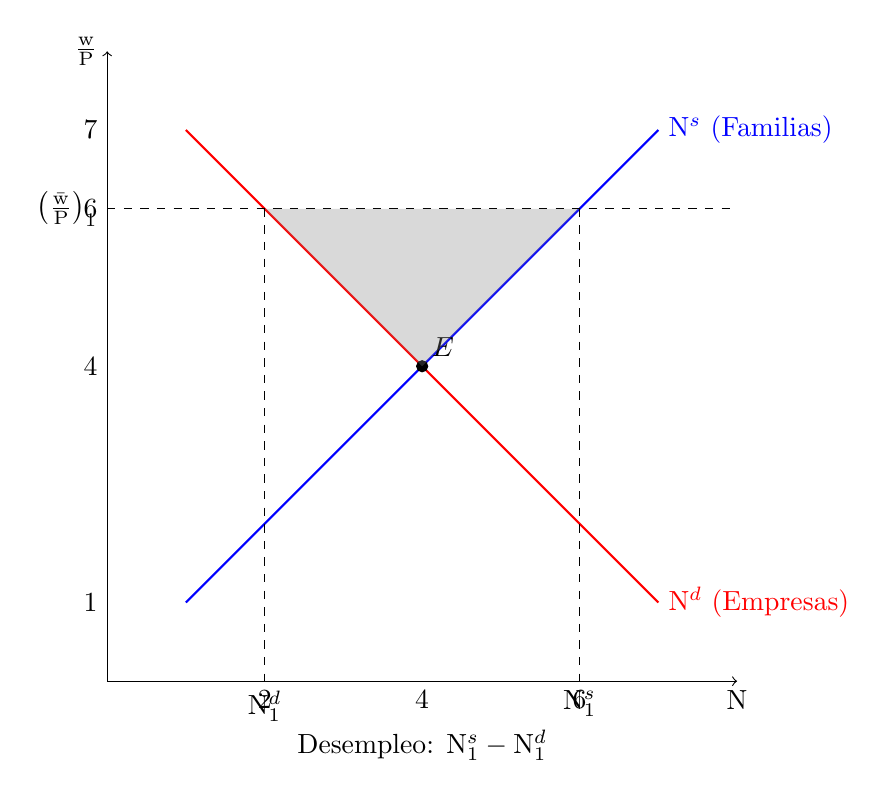
\begin{tikzpicture}
% Ejes
\draw[->] (0,0) -- (8,0) node[below] {$\mathrm{N}$}; % Eje horizontal (Cantidad de trabajo)
\draw[->] (0,0) -- (0,8) node[left] {$\frac{\mathrm{w}}{\mathrm{P}}$}; % Eje vertical (Salario real)
% Curva de oferta de trabajo (N^s): pendiente positiva
\draw[thick, blue] (1,1) -- (7,7) node[right] {$\mathrm{N}^s$ (Familias)};
% Curva de demanda de trabajo (N^d): pendiente negativa
\draw[thick, red] (1,7) -- (7,1) node[right] {$\mathrm{N}^d$ (Empresas)};
% Salario mínimo que genera desequilibrio (w/P = 6)
\draw[dashed] (0,6) node[left] {$\left(\frac{\bar{\mathrm{w}}}{\mathrm{P}}\right)_1$} -- (8,6);
% Puntos de oferta y demanda en el salario mínimo
\draw[dashed] (2,6) -- (2,0) node[below] {$\mathrm{N}^d_1$}; % Demanda
\draw[dashed] (6,6) -- (6,0) node[below] {$\mathrm{N}^s_1$}; % Oferta
% Punto de intersección teórico (equilibrio sin salario mínimo)
\draw[fill=black] (4,4) circle (2pt) node[above right] {$E$}; % Intersección N^s y N^d
% Área triangular sombreada (por debajo del salario mínimo, entre N^s y N^d)
\fill[gray, opacity=0.3] (2,6) -- (4,4) -- (6,6) -- cycle;
% Etiqueta de desempleo
\node[below, align=center] at (4,-0.5) {Desempleo: $\mathrm{N}^s_1 - \mathrm{N}^d_1$};
% Marcas en los ejes
\draw (0,1) node[left] {$1$};
\draw (0,4) node[left] {$4$};
\draw (0,6) node[left] {$6$};
\draw (0,7) node[left] {$7$};
\draw (2,0) node[below] {$2$};
\draw (4,0) node[below] {$4$};
\draw (6,0) node[below] {$6$};
\end{tikzpicture}


\section{Modelo 3: Rigideces Reales (Desempleo Clásico - Salario Real
Rígido)}\label{modelo-3-rigideces-reales-desempleo-cluxe1sico---salario-real-ruxedgido}

El salario real es rígido y está dado por:

\[
\frac{W}{P} = X \quad (\text{rigidez de salario real}).
\]

\subsection{Supuestos}\label{supuestos-2}

\begin{itemize}
\tightlist
\item
  Existe desempleo involuntario debido a un salario real \(X\) por
  encima del nivel que garantiza el equilibrio en el mercado de trabajo
  (\(N^s > N^d\)).
\item
  Equilibrio en el mercado de bienes: \(Y^t = Y^d\).
\item
  Equilibrio en el mercado monetario: \(M^d = M^s\).
\item
  Bajo el supuesto de que, ante una política económica, las variables
  reales (\(Y^t\), \(N^t\)) se comportan de manera contracíclica a las
  variables nominales (\(P\)). Además, el salario real está por encima
  del nivel que vacía el mercado de trabajo, lo que genera desempleo.
\end{itemize}

\[
\frac{dY^t}{dX} < 0, \quad \frac{dN^t}{dX} < 0, \quad \frac{dP}{dX} > 0.
\]

\[
\begin{aligned}
\frac{W}{P} &= X \quad \Rightarrow \text{rígido}, \\
N^t &= N^d(X), \\
Y^t &= Y^s = Y^d, \\
M^d &= M^s.
\end{aligned}
\]

\subsection{Planteamiento del Modelo}\label{planteamiento-del-modelo}

\begin{enumerate}
\def\labelenumi{\arabic{enumi}.}
\item
  \textbf{Ecuaciones del modelo:}

  \[
  \begin{aligned}
  Y^t &= C(Y^t - \bar{T}) + I(r - \bar{\pi}) + \bar{\mathrm{SD}}, \quad \bar{\mathrm{SD}} = \bar{I} + \bar{C} + \bar{G}, \\
  \frac{\bar{M}}{P} &= L(Y^t, r), \\
  N^t &= N^d(X), \\
  Y^t &= f(\bar{K}, N^t).
  \end{aligned}
  \]

  \textbf{Variables endógenas:} \(Y^t\), \(r\), \(N^t\), \(P\).

  \textbf{Variables exógenas:} \(\bar{\mathrm{SD}}\), \(\bar{M}\),
  \(X\), \(\bar{K}\), \(\bar{T}\), \(\bar{\pi}\).
\item
  \textbf{Forma de identidad:}

  Reescribimos las ecuaciones como identidades:

  \[
  \begin{aligned}
  Y^t - C(Y^t - \bar{T}) - I(r - \bar{\pi}) - \bar{\mathrm{SD}} &= 0, \\
  \frac{\bar{M}}{P} - L(Y^t, r) &= 0, \\
  N^t - N^d(X) &= 0, \\
  Y^t - f(\bar{K}, N^t) &= 0.
  \end{aligned}
  \]

  Las variables endógenas dependen funcionalmente de las exógenas:

  \[
  \begin{aligned}
  \tilde{Y}^t &= Y^t(\bar{\mathrm{SD}}, \bar{\pi}, \bar{M}, X), \\
  \tilde{r} &= r(\bar{\mathrm{SD}}, \bar{\pi}, \bar{M}, X), \\
  \tilde{P} &= P(\bar{\mathrm{SD}}, \bar{\pi}, \bar{M}, X), \\
  \tilde{N}^t &= N^t(\bar{\mathrm{SD}}, \bar{\pi}, \bar{M}, X).
  \end{aligned}
  \]
\item
  \textbf{Diferenciales:}

  Tomamos la diferencial total de cada ecuación:

  \[
  \begin{aligned}
  (1 - C_{Y^t}) dY^t - I_r dr &= d\bar{\mathrm{SD}} + I_r d\bar{\pi}, \\
  L_{Y^t} dY^t + L_r dr + \frac{\bar{M}}{P^2} dP &= \frac{1}{P} d\bar{M}, \\
  dN^t &= N^d_X dX, \\
  dY^t - f'(N^t) dN^t &= 0.
  \end{aligned}
  \]
\item
  \textbf{Representación matricial:}

  Escribimos el sistema en forma matricial
  \(\mathbf{A} \mathbf{x} = \mathbf{B} \mathbf{z}\):

  \[
  \begin{bmatrix}
  1 - C_{Y^t} & -I_r & 0 & 0 \\
  L_{Y^t} & L_r & \frac{\bar{M}}{P^2} & 0 \\
  0 & 0 & 0 & 1 \\
  1 & 0 & 0 & -f'(N^t)
  \end{bmatrix}
  \begin{bmatrix}
  dY^t \\
  dr \\
  dP \\
  dN^t
  \end{bmatrix}
  =
  \begin{bmatrix}
  1 & I_r & 0 & 0 \\
  0 & 0 & \frac{1}{P} & 0 \\
  0 & 0 & 0 & N^d_X \\
  0 & 0 & 0 & 0
  \end{bmatrix}
  \begin{bmatrix}
  d\bar{\mathrm{SD}} \\
  d\bar{\pi} \\
  d\bar{M} \\
  dX
  \end{bmatrix}.
  \]
\item
  \textbf{Cálculo del determinante:}

  La matriz \(\mathbf{A}\) es:

  \[
  \mathbf{A} = \begin{bmatrix}
  1 - C_{Y^t} & -I_r & 0 & 0 \\
  L_{Y^t} & L_r & \frac{\bar{M}}{P^2} & 0 \\
  0 & 0 & 0 & 1 \\
  1 & 0 & 0 & -f'(N^t)
  \end{bmatrix}.
  \]

  Calculamos \(\det(\mathbf{A})\) expandiendo por la tercera columna:

  \[
  \det(\mathbf{A}) = \frac{\bar{M}}{P^2} \cdot (-1)^{2+3} \det \begin{bmatrix}
  1 - C_{Y^t} & -I_r & 0 \\
  0 & 0 & 1 \\
  1 & 0 & -f'(N^t)
  \end{bmatrix} + 1 \cdot (-1)^{4+4} \det \begin{bmatrix}
  1 - C_{Y^t} & -I_r & 0 \\
  L_{Y^t} & L_r & \frac{\bar{M}}{P^2} \\
  1 & 0 & 0
  \end{bmatrix}.
  \]

  El primer determinante es 0 (dos filas proporcionales), así que:

  \[
  \det(\mathbf{A}) = \det \begin{bmatrix}
  1 - C_{Y^t} & -I_r & 0 \\
  L_{Y^t} & L_r & \frac{\bar{M}}{P^2} \\
  1 & 0 & 0
  \end{bmatrix}.
  \]

  Expandimos por la tercera fila:

  \[
  \det = 1 \cdot \det \begin{bmatrix}
  -I_r & 0 \\
  L_r & \frac{\bar{M}}{P^2}
  \end{bmatrix} = -I_r \cdot \frac{\bar{M}}{P^2}.
  \]

  Dado que \(I_r < 0\), \(\bar{M} > 0\), \(P > 0\), entonces:

  \[
  \det(\mathbf{A}) = -I_r \frac{\bar{M}}{P^2} > 0.
  \]
\item
  \textbf{Análisis del multiplicador \(\frac{dN^t}{dX}\):}

  Consideramos \(dX \neq 0\), \(d\bar{\mathrm{SD}} = 0\),
  \(d\bar{\pi} = 0\), \(d\bar{M} = 0\):

  \[
  \begin{bmatrix}
  1 - C_{Y^t} & -I_r & 0 & 0 \\
  L_{Y^t} & L_r & \frac{\bar{M}}{P^2} & 0 \\
  0 & 0 & 0 & 1 \\
  1 & 0 & 0 & -f'(N^t)
  \end{bmatrix}
  \begin{bmatrix}
  \frac{dY^t}{dX} \\
  \frac{dr}{dX} \\
  \frac{dP}{dX} \\
  \frac{dN^t}{dX}
  \end{bmatrix}
  =
  \begin{bmatrix}
  0 \\
  0 \\
  N^d_X \\
  0
  \end{bmatrix}.
  \]

  Usamos el método de Cramer:

  \[
  \frac{dN^t}{dX} = \frac{\det(\mathbf{A}_{dN^t})}{\det(\mathbf{A})},
  \]

  donde:

  \[
  \mathbf{A}_{dN^t} = \begin{bmatrix}
  1 - C_{Y^t} & -I_r & 0 & 0 \\
  L_{Y^t} & L_r & \frac{\bar{M}}{P^2} & 0 \\
  0 & 0 & 0 & N^d_X \\
  1 & 0 & 0 & 0
  \end{bmatrix}.
  \]

  Calculamos el determinante expandiendo por la tercera columna:

  \[
  \det(\mathbf{A}_{dN^t}) = N^d_X \cdot (-1)^{3+4} \det \begin{bmatrix}
  1 - C_{Y^t} & -I_r & 0 \\
  L_{Y^t} & L_r & \frac{\bar{M}}{P^2} \\
  1 & 0 & 0
  \end{bmatrix}.
  \]

  Usamos el determinante ya calculado:

  \[
  \det(\mathbf{A}_{dN^t}) = -N^d_X \cdot \left( -I_r \frac{\bar{M}}{P^2} \right) = N^d_X I_r \frac{\bar{M}}{P^2}.
  \]

  Entonces:

  \[
  \frac{dN^t}{dX} = \frac{N^d_X I_r \frac{\bar{M}}{P^2}}{-I_r \frac{\bar{M}}{P^2}} = -N^d_X.
  \]

  Dado que \(N^d_X < 0\) (la demanda de trabajo disminuye con un mayor
  salario real), entonces:

  \[
  \frac{dN^t}{dX} < 0.
  \]

  Esto es consistente con el modelo clásico con rigidez de salario real:
  un aumento en \(X\) reduce el empleo \(N^t\).
\item
  \textbf{Análisis del multiplicador \(\frac{dr}{dX}\):}

  Calculamos el efecto de un cambio en el salario real rígido (\(X\))
  sobre la tasa de interés (\(r\)):

  \[
  \frac{dr}{dX} = \frac{\det(\mathbf{A}_{dr})}{\det(\mathbf{A})},
  \]

  donde:

  \[
  \mathbf{A}_{dr} = \begin{bmatrix}
  1 - C_{Y^t} & 0 & 0 & 0 \\
  L_{Y^t} & N^d_X & \frac{\bar{M}}{P^2} & 0 \\
  0 & 0 & 0 & 1 \\
  1 & 0 & 0 & -f'(N^t)
  \end{bmatrix}.
  \]

  Calculamos el determinante expandiendo por la tercera columna:

  \[
  \det(\mathbf{A}_{dr}) = 0 \cdot (\text{cofactor}) + 1 \cdot (-1)^{4+4} \det \begin{bmatrix}
  1 - C_{Y^t} & 0 & 0 \\
  L_{Y^t} & N^d_X & \frac{\bar{M}}{P^2} \\
  1 & 0 & 0
  \end{bmatrix}.
  \]

  El determinante es:

  \[
  \det \begin{bmatrix}
  1 - C_{Y^t} & 0 & 0 \\
  L_{Y^t} & N^d_X & \frac{\bar{M}}{P^2} \\
  1 & 0 & 0
  \end{bmatrix} = 0,
  \]

  ya que la tercera columna tiene ceros en la primera y tercera filas.
  Entonces:

  \[
  \frac{dr}{dX} = \frac{0}{-I_r \frac{\bar{M}}{P^2}} = 0.
  \]

  Esto indica que un cambio en el salario real rígido no afecta la tasa
  de interés, lo que es consistente con el modelo.
\item
  \textbf{Análisis del multiplicador \(\frac{dY^t}{dX}\):}

  \[
  \frac{dY^t}{dX} = \frac{\det(\mathbf{A}_{dY^t})}{\det(\mathbf{A})},
  \]

  donde:

  \[
  \mathbf{A}_{dY^t} = \begin{bmatrix}
  0 & -I_r & 0 & 0 \\
  0 & L_r & \frac{\bar{M}}{P^2} & 0 \\
  N^d_X & 0 & 0 & 1 \\
  0 & 0 & 0 & -f'(N^t)
  \end{bmatrix}.
  \]

  Calculamos el determinante:

  \[
  \det(\mathbf{A}_{dY^t}) = 0 \cdot (\text{cofactor}) + (-f'(N^t)) \cdot (-1)^{4+4} \det \begin{bmatrix}
  0 & -I_r & 0 \\
  0 & L_r & \frac{\bar{M}}{P^2} \\
  N^d_X & 0 & 0
  \end{bmatrix}.
  \]

  El determinante del bloque es:

  \[
  \det \begin{bmatrix}
  0 & -I_r & 0 \\
  0 & L_r & \frac{\bar{M}}{P^2} \\
  N^d_X & 0 & 0
  \end{bmatrix} = N^d_X \cdot (-1)^{3+1} \det \begin{bmatrix}
  -I_r & 0 \\
  L_r & \frac{\bar{M}}{P^2}
  \end{bmatrix} = N^d_X \cdot (-I_r) \cdot \frac{\bar{M}}{P^2}.
  \]

  Entonces:

  \[
  \det(\mathbf{A}_{dY^t}) = -f'(N^t) \cdot N^d_X \cdot (-I_r) \cdot \frac{\bar{M}}{P^2} = f'(N^t) N^d_X I_r \frac{\bar{M}}{P^2}.
  \]

  Por lo tanto:

  \[
  \frac{dY^t}{dX} = \frac{f'(N^t) N^d_X I_r \frac{\bar{M}}{P^2}}{-I_r \frac{\bar{M}}{P^2}} = f'(N^t) N^d_X.
  \]

  Dado que \(f'(N^t) > 0\) y \(N^d_X < 0\), entonces:

  \[
  \frac{dY^t}{dX} < 0.
  \]
\item
  \textbf{Análisis del multiplicador \(\frac{dP}{dX}\):}

  \[
  \frac{dP}{dX} = \frac{\det(\mathbf{A}_{dP})}{\det(\mathbf{A})},
  \]

  donde:

  \[
  \mathbf{A}_{dP} = \begin{bmatrix}
  1 - C_{Y^t} & -I_r & 0 & 0 \\
  L_{Y^t} & L_r & N^d_X & 0 \\
  0 & 0 & 0 & 1 \\
  1 & 0 & 0 & -f'(N^t)
  \end{bmatrix}.
  \]

  Calculamos el determinante:

  \[
  \det(\mathbf{A}_{dP}) = N^d_X \cdot (-1)^{2+3} \det \begin{bmatrix}
  1 - C_{Y^t} & -I_r & 0 \\
  0 & 0 & 1 \\
  1 & 0 & -f'(N^t)
  \end{bmatrix} + 1 \cdot (-1)^{4+4} \det \begin{bmatrix}
  1 - C_{Y^t} & -I_r & 0 \\
  L_{Y^t} & L_r & N^d_X \\
  1 & 0 & 0
  \end{bmatrix}.
  \]

  El primer determinante es 0, y el segundo es:

  \[
  \det \begin{bmatrix}
  1 - C_{Y^t} & -I_r & 0 \\
  L_{Y^t} & L_r & N^d_X \\
  1 & 0 & 0
  \end{bmatrix} = -N^d_X \cdot \det \begin{bmatrix}
  1 - C_{Y^t} & -I_r \\
  1 & 0
  \end{bmatrix} = -N^d_X \cdot (-I_r) = N^d_X I_r.
  \]

  Entonces:

  \[
  \frac{dP}{dX} = \frac{N^d_X I_r}{-I_r \frac{\bar{M}}{P^2}} = -\frac{N^d_X}{\frac{\bar{M}}{P^2}}.
  \]

  Dado que \(N^d_X < 0\), \(\bar{M} > 0\), \(P > 0\), entonces:

  \[
  \frac{dP}{dX} > 0.
  \]
\end{enumerate}

\section{Modelo 4: Rigideces Reales y Nominales (Desempleo
Keynesiano)}\label{modelo-4-rigideces-reales-y-nominales-desempleo-keynesiano}

\subsection{Supuestos}\label{supuestos-3}

\begin{itemize}
\tightlist
\item
  \textbf{Precios y salarios rígidos:} \(\bar{P}\) y \(\bar{W}\).
\item
  \textbf{Dos fallas de mercado:}

  \begin{itemize}
  \tightlist
  \item
    Exceso de oferta de bienes: \(Y^s > Y^d = Y^t\).
  \item
    Exceso de oferta de trabajo: \(N^s > N^d = N^t\).
  \end{itemize}
\item
  \textbf{Función de producción inversa:} \(N^t = F^{-1}(Y^d)\).
\item
  Las empresas no venden toda su producción a los precios vigentes, por
  lo que no contratan más trabajadores aunque el salario disminuya.
\end{itemize}

\subsection{Modelo Resumen}\label{modelo-resumen}

\[
\begin{aligned}
Y^t &= C(Y^t - \bar{T}) + I(r) + \bar{\mathrm{SD}}, \\
\frac{\bar{M}}{\bar{P}} &= L(Y^t, r), \\
N^t &= F^{-1}(Y^t).
\end{aligned}
\]

\textbf{Variables endógenas:} \(Y^t\), \(r\), \(N^t\).

\textbf{Variables exógenas:} \(\bar{\mathrm{SD}}\), \(\bar{M}\),
\(\bar{W}/\bar{P}\), \(\bar{T}\).

\subsection{Planteamiento del Modelo}\label{planteamiento-del-modelo-1}

\begin{enumerate}
\def\labelenumi{\arabic{enumi}.}
\item
  \textbf{Ecuaciones:}

  \[
  \begin{aligned}
  Y^t &= C(Y^t - \bar{T}) + I(r) + \bar{\mathrm{SD}}, \\
  \frac{\bar{M}}{\bar{P}} &= L(Y^t, r), \\
  N^t &= F^{-1}(Y^t).
  \end{aligned}
  \]
\item
  \textbf{Forma de identidad:}

  \[
  \begin{aligned}
  Y^t - C(Y^t - \bar{T}) - I(r) - \bar{\mathrm{SD}} &= 0, \\
  \frac{\bar{M}}{\bar{P}} - L(Y^t, r) &= 0, \\
  N^t - F^{-1}(Y^t) &= 0.
  \end{aligned}
  \]

  Las variables endógenas dependen de las exógenas:

  \[
  \begin{aligned}
  Y^{t*} &= Y^t(\bar{\mathrm{SD}}, \bar{M}, \bar{W}/\bar{P}, \bar{T}), \\
  r^* &= r(\bar{\mathrm{SD}}, \bar{M}, \bar{W}/\bar{P}, \bar{T}), \\
  N^{t*} &= N^t(\bar{\mathrm{SD}}, \bar{M}, \bar{W}/\bar{P}, \bar{T}).
  \end{aligned}
  \]
\item
  \textbf{Diferenciales:}

  \[
  \begin{aligned}
  (1 - C_{Y^t}) dY^t - I_r dr &= d\bar{\mathrm{SD}} - C_T d\bar{T}, \\
  -L_{Y^t} dY^t - L_r dr &= -\frac{1}{\bar{P}} d\bar{M}, \\
  dN^t - (F^{-1})'(Y^t) dY^t &= 0.
  \end{aligned}
  \]
\item
  \textbf{Matriz:}

  \[
  \begin{bmatrix}
  1 - C_{Y^t} & -I_r & 0 \\
  -L_{Y^t} & -L_r & 0 \\
  -(F^{-1})'(Y^t) & 0 & 1
  \end{bmatrix}
  \begin{bmatrix}
  dY^t \\
  dr \\
  dN^t
  \end{bmatrix}
  =
  \begin{bmatrix}
  1 & 0 & -C_T & 0 \\
  0 & -\frac{1}{\bar{P}} & 0 & 0 \\
  0 & 0 & 0 & 0
  \end{bmatrix}
  \begin{bmatrix}
  d\bar{\mathrm{SD}} \\
  d\bar{M} \\
  d\bar{T} \\
  d(\bar{W}/\bar{P})
  \end{bmatrix}.
  \]
\item
  \textbf{Determinante:}

  \[
  \Delta = \begin{vmatrix}
  1 - C_{Y^t} & -I_r & 0 \\
  -L_{Y^t} & -L_r & 0 \\
  -(F^{-1})'(Y^t) & 0 & 1
  \end{vmatrix}.
  \]

  Expandiendo por la tercera columna:

  \[
  \Delta = 1 \cdot \det \begin{bmatrix}
  1 - C_{Y^t} & -I_r \\
  -L_{Y^t} & -L_r
  \end{bmatrix} = (1 - C_{Y^t})(-L_r) - (-I_r)(-L_{Y^t}) = L_r (1 - C_{Y^t}) + I_r L_{Y^t}.
  \]

  Dado que \(L_r < 0\), \(I_r < 0\), \(L_{Y^t} > 0\),
  \(1 - C_{Y^t} > 0\), entonces \(\Delta > 0\).
\item
  \textbf{Política monetaria:}

  Consideramos \(d\bar{M} \neq 0\), \(d\bar{\mathrm{SD}} = 0\),
  \(d\bar{T} = 0\), \(d(\bar{W}/\bar{P}) = 0\):

  \[
  \begin{bmatrix}
  1 - C_{Y^t} & -I_r & 0 \\
  -L_{Y^t} & -L_r & 0 \\
  -(F^{-1})'(Y^t) & 0 & 1
  \end{bmatrix}
  \begin{bmatrix}
  \frac{dY^t}{d\bar{M}} \\
  \frac{dr}{d\bar{M}} \\
  \frac{dN^t}{d\bar{M}}
  \end{bmatrix}
  =
  \begin{bmatrix}
  0 \\
  -\frac{1}{\bar{P}} \\
  0
  \end{bmatrix}.
  \]

  Calculamos \(\frac{dY^t}{d\bar{M}}\):

  \[
  \frac{dY^t}{d\bar{M}} = \frac{\det \begin{bmatrix}
  0 & -I_r & 0 \\
  -\frac{1}{\bar{P}} & -L_r & 0 \\
  0 & 0 & 1
  \end{bmatrix}}{\Delta}.
  \]

  Numerador:

  \[
  \det \begin{bmatrix}
  0 & -I_r & 0 \\
  -\frac{1}{\bar{P}} & -L_r & 0 \\
  0 & 0 & 1
  \end{bmatrix} = 1 \cdot \det \begin{bmatrix}
  0 & -I_r \\
  -\frac{1}{\bar{P}} & -L_r
  \end{bmatrix} = -I_r \cdot \frac{1}{\bar{P}}.
  \]

  Entonces:

  \[
  \frac{dY^t}{d\bar{M}} = \frac{-\frac{I_r}{\bar{P}}}{L_r (1 - C_{Y^t}) + I_r L_{Y^t}}.
  \]

  Dado que \(I_r < 0\), \(\bar{P} > 0\), y \(\Delta > 0\), entonces:

  \[
  \frac{dY^t}{d\bar{M}} > 0.
  \]

  Calculamos \(\frac{dN^t}{d\bar{M}}\):

  \[
  \frac{dN^t}{d\bar{M}} = \frac{\det \begin{bmatrix}
  1 - C_{Y^t} & -I_r & 0 \\
  -L_{Y^t} & -L_r & -\frac{1}{\bar{P}} \\
  -(F^{-1})'(Y^t) & 0 & 0
  \end{bmatrix}}{\Delta}.
  \]

  Numerador:

  \[
  \det \begin{bmatrix}
  1 - C_{Y^t} & -I_r & 0 \\
  -L_{Y^t} & -L_r & -\frac{1}{\bar{P}} \\
  -(F^{-1})'(Y^t) & 0 & 0
  \end{bmatrix} = -(F^{-1})'(Y^t) \cdot (-1)^{3+3} \det \begin{bmatrix}
  -I_r & 0 \\
  -L_r & -\frac{1}{\bar{P}}
  \end{bmatrix}.
  \]

  Calculando:

  \[
  \det \begin{bmatrix}
  -I_r & 0 \\
  -L_r & -\frac{1}{\bar{P}}
  \end{bmatrix} = (-I_r) \cdot \left(-\frac{1}{\bar{P}}\right) = \frac{I_r}{\bar{P}}.
  \]

  Entonces:

  \[
  \det = -(F^{-1})'(Y^t) \cdot \frac{I_r}{\bar{P}} = -(F^{-1})'(Y^t) \frac{I_r}{\bar{P}}.
  \]

  Por lo tanto:

  \[
  \frac{dN^t}{d\bar{M}} = \frac{-(F^{-1})'(Y^t) \frac{I_r}{\bar{P}}}{L_r (1 - C_{Y^t}) + I_r L_{Y^t}}.
  \]

  Dado que \((F^{-1})'(Y^t) > 0\), \(I_r < 0\), \(\bar{P} > 0\), y
  \(\Delta > 0\), entonces:

  \[
  \frac{dN^t}{d\bar{M}} > 0.
  \]

  Esto indica que una política monetaria expansiva (\(d\bar{M} > 0\))
  aumenta la producción (\(Y^t\)) y el empleo (\(N^t\)), comportándose
  de manera procíclica con las variables reales y contracíclica con la
  tasa de interés (si \(dr/d\bar{M} < 0\)).
\end{enumerate}

\section{Publicaciones Similares}\label{publicaciones-similares}

Si te interesó este artículo, te recomendamos que explores otros blogs y
recursos relacionados que pueden ampliar tus conocimientos. Aquí te dejo
algunas sugerencias:

\begin{enumerate}
\def\labelenumi{\arabic{enumi}.}
\tightlist
\item
  \href{https://achalmaedison.netlify.app/matematicas/posts/2024-03-31-por-editar/index.pdf}{\faIcon{file-pdf}}
  \href{https://achalmaedison.netlify.app/matematicas/posts/2024-03-31-por-editar}{Por
  Editar}
\end{enumerate}

Esperamos que encuentres estas publicaciones igualmente interesantes y
útiles. ¡Disfruta de la lectura!






\end{document}
